\documentclass[a4paper,twoside,12pt]{article}
\usepackage[top=1.5cm,left=1.5cm,right=1.5cm,bottom=2cm]{geometry}

\usepackage[utf8]{inputenc}
\usepackage[T1]{fontenc}
\usepackage{lmodern}
\usepackage[brazilian]{babel}

\usepackage{graphicx}
\usepackage{subfig}
\usepackage{psfrag}
\usepackage{cite}
\usepackage[cmex10]{amsmath}
\usepackage{amssymb}
\usepackage{upgreek}
\usepackage{microtype}
\usepackage{titling}
\usepackage{courier}
\usepackage{url}
\usepackage{hyperref}
\hypersetup{
	colorlinks=true,
	linkcolor=blue,
	urlcolor=blue
}

% Use o pacote 'listings' para adicionar código e o pacote 'color' para gerar os destaques
\usepackage{listings}
\usepackage{color}
\definecolor{grey}{rgb}{0.6,0.6,0.6}
\definecolor{codegreen}{rgb}{0,0.6,0}
\definecolor{codegray}{rgb}{0.5,0.5,0.5}
\definecolor{codepurple}{rgb}{0.58,0,0.82}
\definecolor{backcolour}{rgb}{0.95,0.95,0.92}
\lstset{language=Python,				% definir para destaque de linguagem Python
	backgroundcolor=\color{backcolour},
	commentstyle=\color{codegreen},
	keywordstyle=\color{magenta},
	numberstyle=\tiny\color{codegray},
	stringstyle=\color{codepurple},
	basicstyle=\ttfamily\small,		% definir tamanho das fontes
	breaklines=true,				% definir quebra de linha automática
	linewidth=\textwidth,			% definir tamanho da caixa de código
	showstringspaces=false}			% mostrar espaços como sublinhados apenas dentro de strings


\title{\vspace{-2cm} Processamento Digital de Sinais\\ Soluções para Tutorial 15 - Modulação AM/FM e Transformada de Hilbert}
\author{\url{https://github.com/fchirono/Aulas_PDS_Acustica}}

\begin{document}
	\date{}
	\maketitle
	
	
	\setcounter{section}{1}
	\section{Tarefas}
	\label{sec:tarefas}
	
	\subsection{Geração dos Sinais Moduladores e Modulados}
	\label{sec:tarefas1}
	
	\subsubsection*{Tarefa 1}
	Veja o script \texttt{tutorial15\_solucoes.py} para um exemplo de como esta Tarefa pode ser solucionada.
	
	\subsubsection*{Tarefa 2}
	
	A função \texttt{gerador\_seno\_am} (no script \texttt{tutorial15\_solucoes.py}) implementa diretamente a Equação (2) do enunciado, com a portadora $x_c(t) = \sin(2\pi f_c t)$ construída sobre um vetor de tempo de mesmo comprimento que \texttt{xmod}. O índice de modulação $m$ é o valor de pico de \texttt{xmod}, e um aviso é emitido sempre que o índice de modulação $m>1$ (sobremodulação).
	
	Esta implementação foi adaptada da função \texttt{mosqito.utils.am\_sine\_generation} do pacote \texttt{MoSQITo}, disponível em \url{https://github.com/Eomys/MoSQITo}.
	
	
	\subsubsection*{Tarefa 3}
	
	A função \texttt{gerador\_seno\_fm} (no script \texttt{tutorial15\_solucoes.py}) implementa a Equação (5), integrando numericamente a frequência instantânea $f_{inst}(t) = f_c + k\, x_{mod}(t)$ por soma acumulada (\texttt{numpy.cumsum}) para obter a fase $\phi(t)$. O desvio máximo de frequência $\Delta f$ e o índice de modulação $\beta$ são calculados diretamente das definições da Seção 1.2 do enunciado.
	
	Esta implementação foi adaptada da função \texttt{mosqito.utils.fm\_sine\_generation} do pacote \texttt{MoSQITo}, disponível em \url{https://github.com/Eomys/MoSQITo}.
	
	\subsubsection*{Tarefa 4}
	
	Utilizando um sinal modulador de banda limitada (Tarefa 1), com portadora $f_c=30$ Hz (para melhor visualização dos resultados neste documento) e sensibilidade em frequência $k=50$ Hz, obtêm-se os sinais AM e FM das Figuras \ref{fig:AM_geracao} e \ref{fig:FM_geracao}. Nota-se claramente a amplitude do sinal AM e a frequência instantânea do sinal FM variando de acordo com o sinal modulador, conforme esperado. 
	
	\begin{figure}[h!]
		\centering
		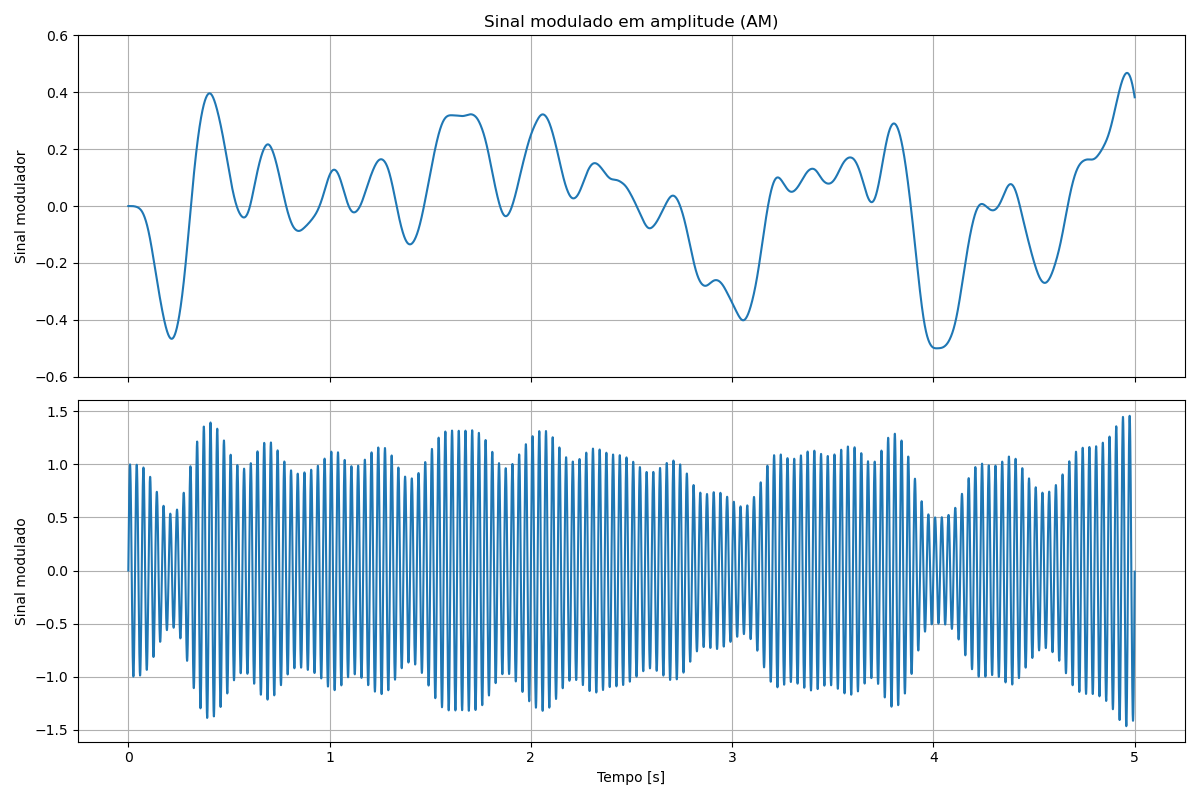
\includegraphics[width=0.85\textwidth]{sinal_AM.png}
		\caption{Sinal modulador de banda limitada (topo), sinal AM completo ($f_c=30$ Hz).}
		\label{fig:AM_geracao}
	\end{figure}
	
	\begin{figure}[h!]
		\centering
		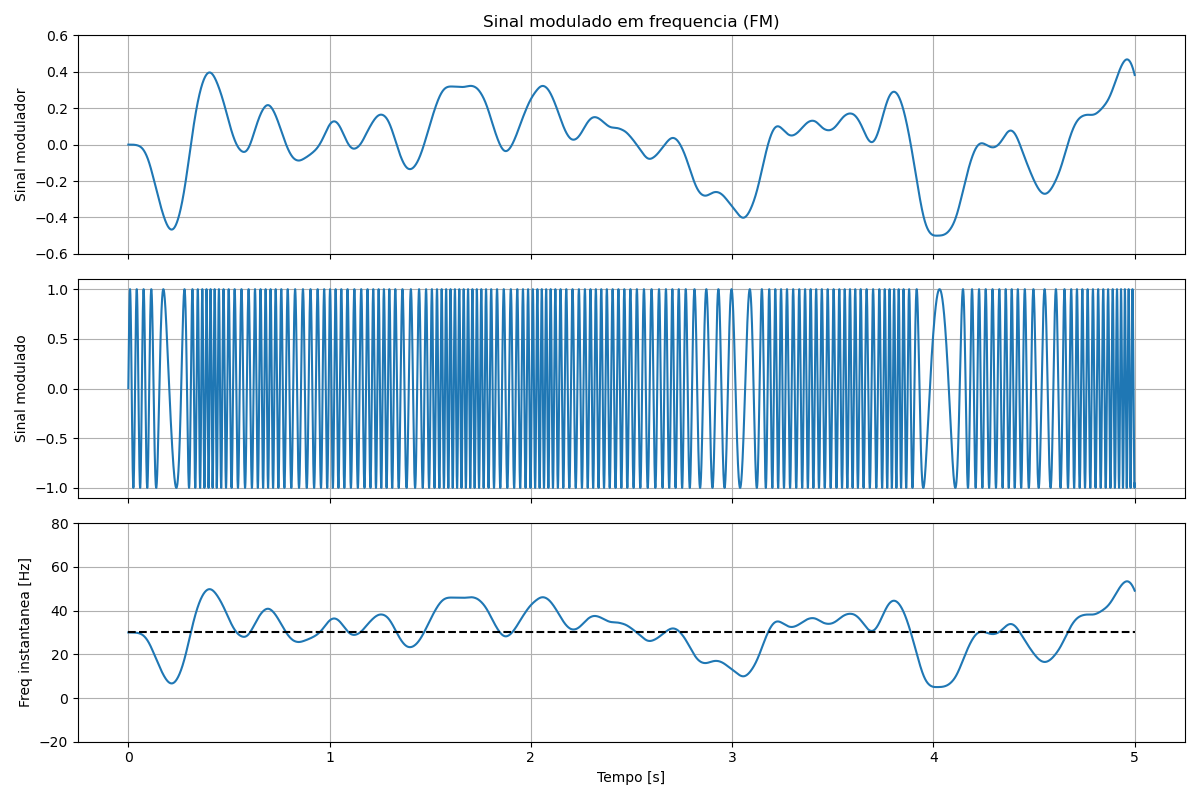
\includegraphics[width=0.85\textwidth]{sinal_FM.png}
		\caption{Sinal modulador de banda limitada (topo), sinal FM ($f_c=30$ Hz), e frequência instantânea $f_{inst}(t)$.}
		\label{fig:FM_geracao}
	\end{figure}
	
	\clearpage
	\newpage
	\subsection{Sinal Analítico via Transformada de Hilbert}
	\label{sec:tarefas2}
	
	\subsubsection*{Tarefa 1}
	
	Uma das principais propriedades do sinal analítico é possuir um espectro \emph{unilateral} -- isto é, contendo apenas frequências positivas (e a componente DC, quando existente). Partindo de $z(t) = x(t) + j\tilde{x}(t)$ e de $H(f) = -j\,\mathrm{sgn}(f)$ (resposta em frequência da Transformada de Hilbert, Equação 6), tem-se $\tilde{X}(f) = H(f)X(f)$, e portanto:
	\begin{align}
		Z(f) &= X(f) + j\, H(f)\, X(f) \nonumber \\
		&= X(f)\left[1 + j\left(-j\,\mathrm{sgn}(f)\right)\right] \nonumber \\
		&= X(f)\left[1 + \mathrm{sgn}(f)\right] \nonumber \\[4pt]
		&= \begin{cases}
			2\, X(f), & f > 0\\
			X(f), & f = 0 \ \mathrm{ou} \ f = f_s/2\\
			0, & f < 0
		\end{cases}.
		\label{eq:Zomega}
	\end{align}
	
	\noindent Ou seja, as componentes de frequência negativa de $X(\Omega)$ são canceladas, as de frequência positiva são dobradas em amplitude, e a componente DC e a frequência de Nyquist $f_s/2$ permanecem inalteradas.
	
	\subsubsection*{Tarefa 2}
	
	Numericamente, o sinal analítico de uma sequência real $x[n]$ de comprimento par $N$ pode ser calculado diretamente no domínio da frequência, explorando a propriedade \eqref{eq:Zomega}: calcula-se a DFT $X[k]$ de $x[n]$, multiplica-se $X[k]$ por um vetor $h[k]$ que implementa a versão discreta de $1+\mathrm{sgn}(\Omega)$,
	\begin{equation}
		h[k] = 
		\begin{cases}
			1, & k = 0 \text{ ou } k = N/2 \quad \text{(DC e Nyquist)}\\
			2, & k = 1, \ldots, N/2 - 1 \quad \text{(frequências positivas)}\\
			0, & k = N/2+1, \ldots, N-1 \quad \text{(frequências negativas)}
		\end{cases},
	\end{equation}
	e retorna-se ao domínio do tempo pela IDFT: $z[n] = \mathrm{IDFT}\left\{X[k]\, h[k]\right\}$. As componentes DC e Nyquist \emph{não} são dobradas, pois são as únicas frequências que não possuem uma componente ``espelhada'' (negativa) distinta a ser descartada.
	
	\begin{lstlisting}[frame=single]
def calc_sinal_analitico(x):
    """
    Retorna o sinal analitico z = x + j*Hilbert(x), calculado no dominio
    da frequencia a partir da propriedade de espectro unilateral.
    """
    N = x.shape[0]
    Xf = np.fft.fft(x)
    
    # vetor 'h[k]' para multiplicar o espectro de 'x'
    h = np.zeros(N)
    
    # frequencia zero (DC) e Nyquist sao multiplicadas por 1
    h[0] = h[N // 2] = 1
    
    # frequencias positivas sao multiplicadas por 2
    h[1 : N // 2] = 2
    
    # frequencias negativas permanecem multiplicadas por 0
    return np.fft.ifft(Xf * h)
	\end{lstlisting}
	
	\noindent \textbf{Nota importante}: o resultado da IDFT é, em geral, complexo -- a parte real reproduz exatamente $x[n]$ (a menos de erro numérico de ponto flutuante), e a parte imaginária é a Transformada de Hilbert $\tilde{x}[n]$.
	
	A Figura \ref{fig:hilbert_comp} compara o sinal analítico de um tom puro $x[n]=\cos(2\pi f_0 n/f_s)$, calculado tanto por \texttt{calc\_sinal\_analitico} quanto pela função de referência \texttt{scipy.signal.hilbert}. As partes real e imaginária das duas implementações coincidem ponto a ponto (erro máximo da ordem de $10^{-15}$, compatível com precisão de ponto flutuante), confirmando que a implementação via DFT é matematicamente equivalente à da biblioteca SciPy.
	
	\begin{figure}[h!]
		\centering
		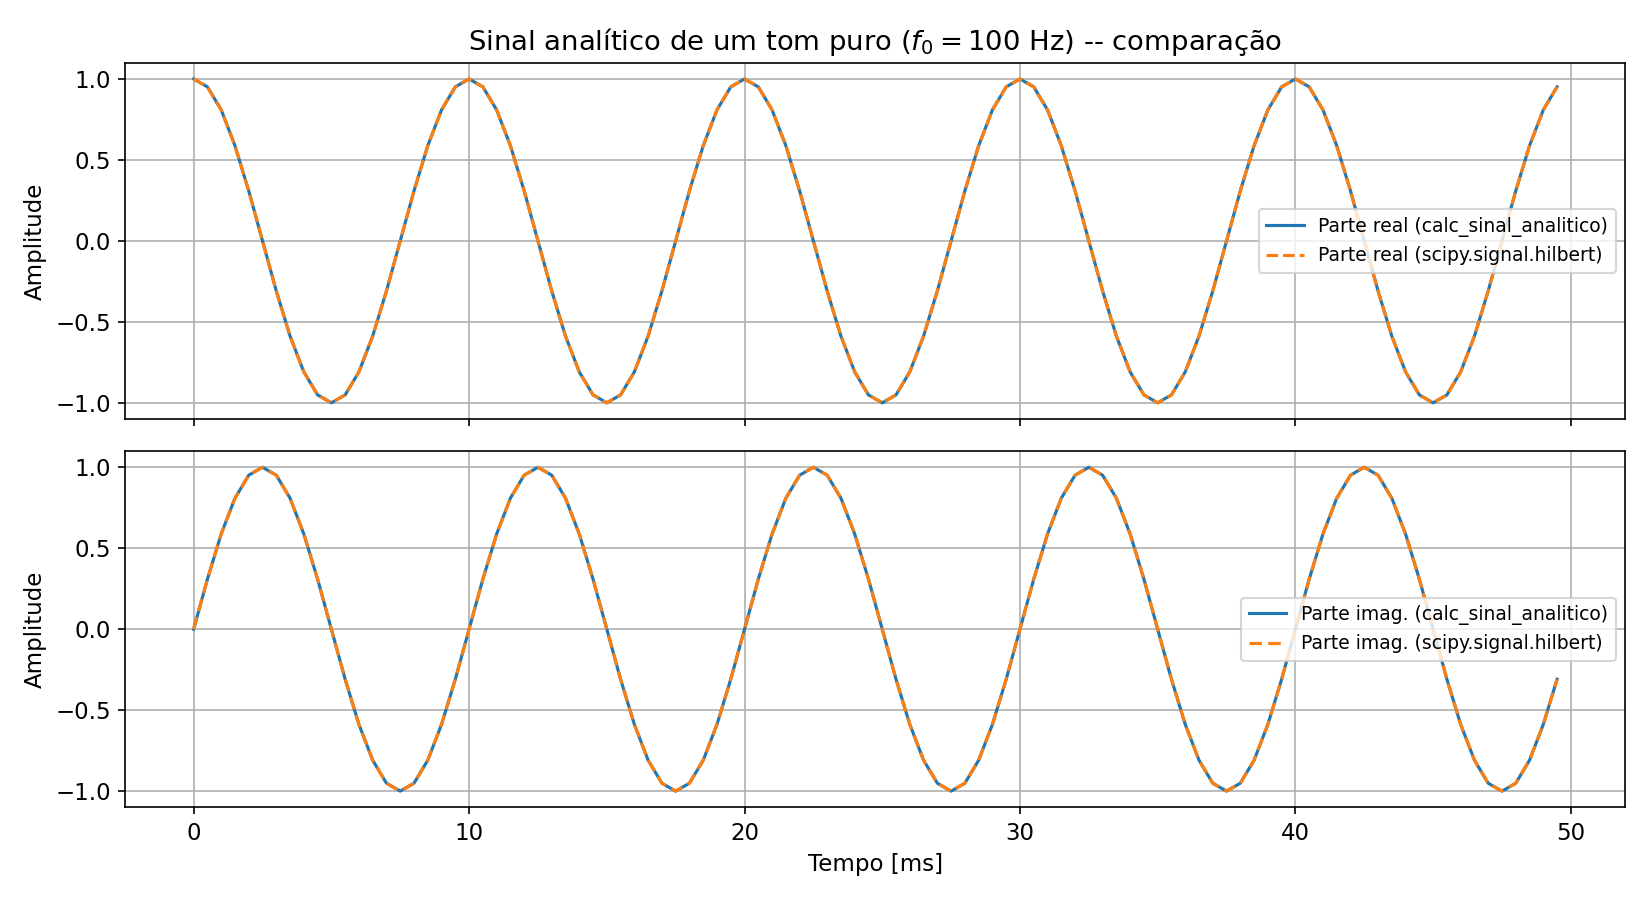
\includegraphics[width=0.85\textwidth]{fig_hilbert_comparacao.png}
		\caption{Partes real (topo) e imaginária (embaixo) do sinal analítico de um tom puro de $100$ Hz, calculado por \texttt{calc\_sinal\_analitico} e por \texttt{scipy.signal.hilbert}. As curvas se sobrepõem perfeitamente.}
		\label{fig:hilbert_comp}
	\end{figure}
	
	\newpage
	\subsection{Demodulação dos Sinais AM e FM}
	\label{sec:tarefas3}
	
	\subsubsection*{Tarefas 1 e 2 -- Demodulação AM}
	
	O sinal analítico do sinal AM é calculado por \texttt{calc\_sinal\_analitico(sinal\_AM)}. Sua magnitude fornece a envoltória, da qual se subtrai o nível DC unitário da portadora para recuperar o sinal modulador (Seção 1.4.1 do enunciado).
	
	A Figura \ref{fig:demod_AM} mostra, no painel superior, o sinal AM (linha sólida azul) sobreposto à envoltória calculada (linha tracejada laranja), e, no painel inferior, o sinal modulador original (linha sólida azul) sobreposto ao sinal modulador recuperado (linha tracejada laranja). A concordância é excelente, e as únicas discrepâncias visíveis ocorrem nas \textbf{bordas} do sinal ($t\approx0$ e $t\approx5$ s), onde aparecem picos espúrios no sinal recuperado.
	
	\begin{figure}[h!]
		\centering
		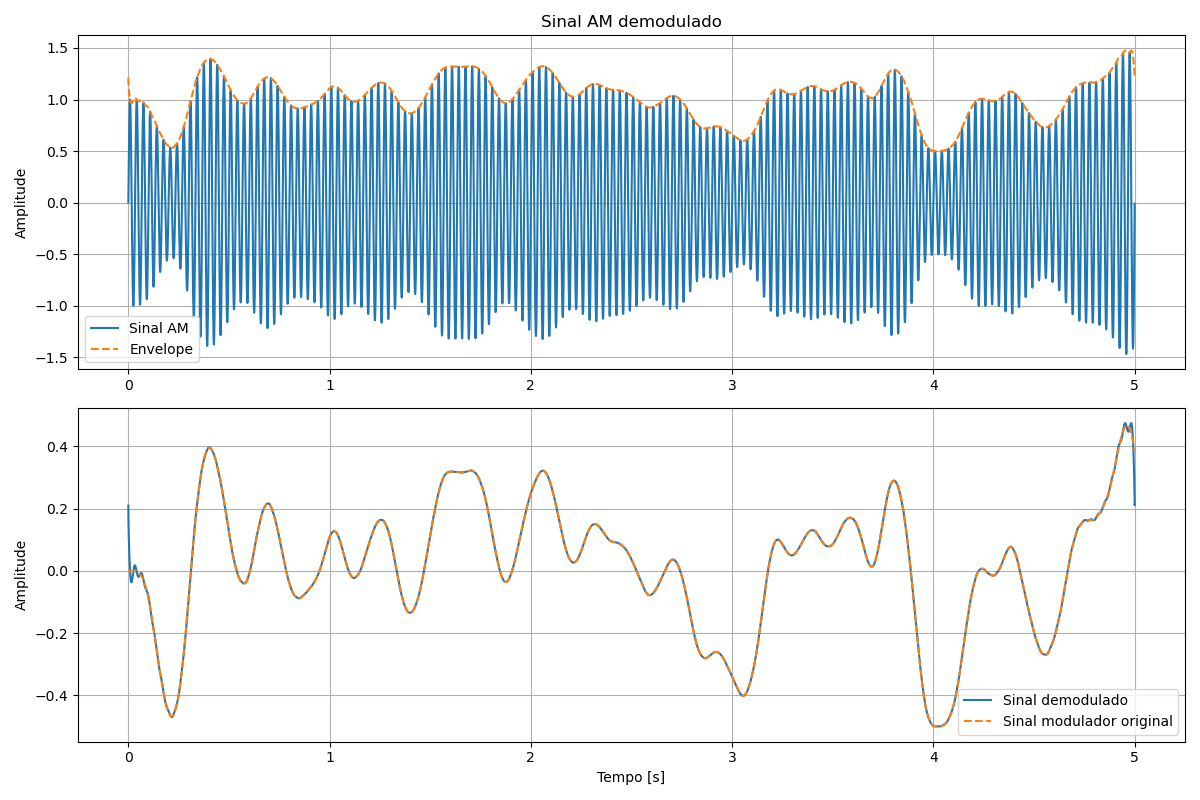
\includegraphics[width=0.85\textwidth]{sinal_AM_demodulado.png}
		\caption{Demodulação AM: sinal AM e envoltória calculada (topo, zoom de 20 ms) e sinal modulador recuperado vs. original (embaixo, sinal completo).}
		\label{fig:demod_AM}
	\end{figure}
	
	Essas discrepâncias nas bordas ocorrem porque \texttt{calc\_sinal\_analitico} é calculado via DFT, que assume implicitamente que o sinal de entrada é \emph{periódico} com período $N$ (o comprimento do sinal). Como o sinal AM real não é periódico -- e portanto, sua primeira e última amostras não se conectam suavemente --, a DFT ``enxerga'' uma descontinuidade artificial na fronteira circular entre o fim e o início do sinal. Essa descontinuidade se manifesta como conteúdo espectral espúrio (efeito de borda, análogo ao \emph{leakage} espectral), que corrompe a estimativa da envoltória justamente nas amostras mais próximas das extremidades do sinal. 
	
	\subsubsection*{Tarefas 3 e 4 -- Demodulação FM}
	
	De forma análoga, o sinal analítico do sinal FM é calculado por \texttt{calc\_sinal\_analitico(sinal\_FM)}. Sua fase, desembrulhada com \texttt{numpy.unwrap}, é diferenciada numericamente para obter a frequência instantânea, da qual se recupera o sinal modulador (Seção 1.4.2 do enunciado). 
		
	A Figura \ref{fig:demod_FM} mostra a frequência instantânea original (linha sólida azul) sobreposta à frequência instantânea recuperada (linha tracejada laranja). Assim como no caso AM, ambos os sinais apresentam excelente concordância, e a única discrepância visível ocorre novamente nas \textbf{bordas} do sinal, pelo mesmo motivo discutido na demodulação AM: a suposição implícita de periodicidade da DFT usada em \texttt{calc\_sinal\_analitico} introduz uma descontinuidade espúria na fronteira circular do sinal, degradando a estimativa da fase (e, por consequência, da frequência instantânea) nas amostras próximas às extremidades.
	
	\begin{figure}[h!]
		\centering
		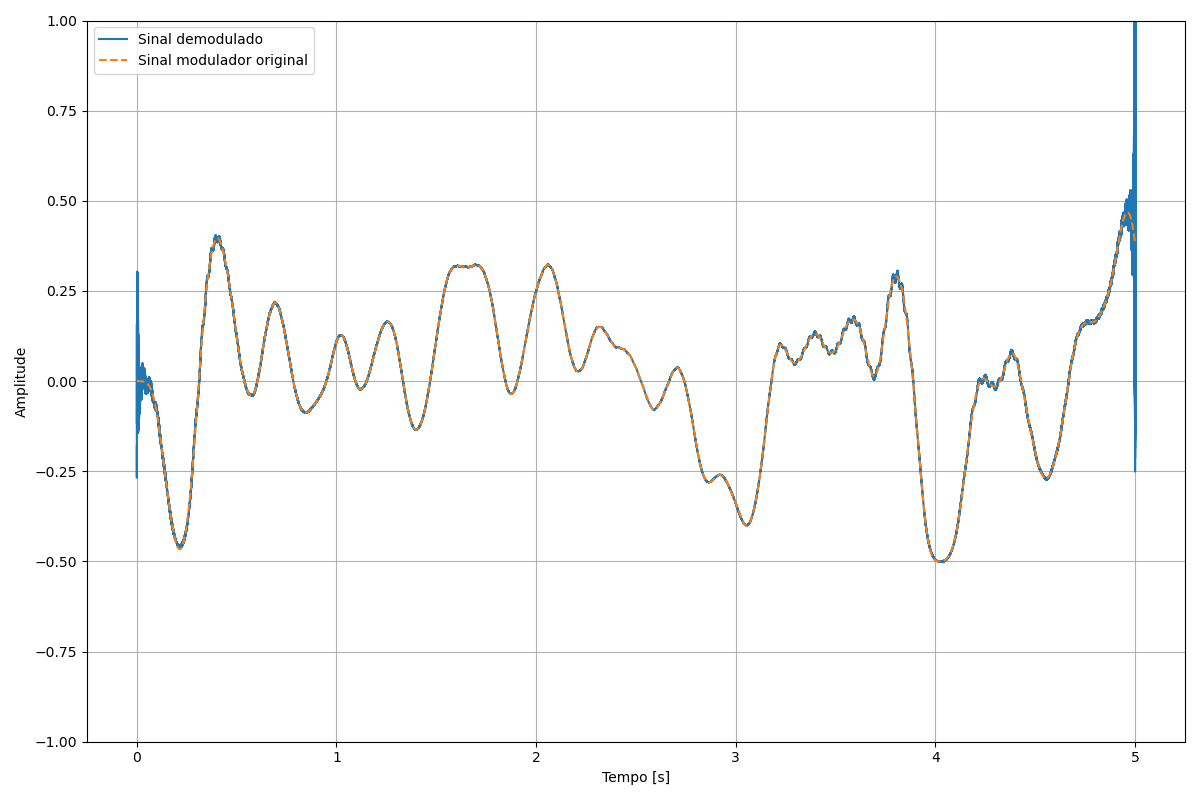
\includegraphics[width=0.85\textwidth]{sinal_FM_demodulado.png}
		\caption{Demodulação FM: frequência instantânea recuperada vs. original, sinal completo (topo) e zoom longe das bordas (meio); sinal modulador recuperado vs. original, sinal completo (embaixo).}
		\label{fig:demod_FM}
	\end{figure}
	
	\noindent \textbf{Sobre o comprimento do vetor de frequência instantânea:} a frequência instantânea é obtida por diferenciação numérica (diferenças finitas) da fase desembrulhada, $f_{inst}[n] \approx \left(\varphi[n+1]-\varphi[n]\right)/(2\pi\Delta t)$. Como essa operação (\texttt{numpy.diff}) calcula a diferença entre pares de amostras \emph{consecutivas}, um vetor de fase com $N$ amostras produz um vetor de diferenças com apenas $N-1$ amostras -- não existe uma amostra ``seguinte'' à última amostra do sinal para calcular a última diferença. Por isso, o vetor \texttt{modulador\_FM} (e o eixo de tempo correspondente, \texttt{t[:-1]}) possui um elemento a menos que o sinal modulador original.
	
	
	% -----------------------------------------------------------------------
	\section*{Referências}
	
	\begin{enumerate}
		\item J. Bendat, A. Piersol, \emph{Random Data: Analysis and Measurement Procedures} (2a Edição), Wiley
		\item Pacote MOSQITO (código de referência para geração dos sinais AM/FM): \url{https://github.com/Eomys/MoSQITo}
	\end{enumerate}
	
\end{document}